\documentclass[12pt]{report}
\usepackage[a4paper,width=150mm,top=25mm,bottom=25mm]{geometry}
\usepackage{graphicx}
\usepackage[utf8]{inputenc}
\usepackage{alphabeta}
\usepackage{hyperref}
\usepackage{textcomp}
\usepackage{listings}
\usepackage{xcolor}
\usepackage{cleveref}

\definecolor{codegreen}{rgb}{0,0.6,0}
\definecolor{codegray}{rgb}{0.5,0.5,0.5}
\definecolor{codepurple}{rgb}{0.58,0,0.82}
\definecolor{backcolour}{rgb}{0.95,0.95,0.92}
\definecolor{mygreen}{rgb}{0,0.6,0}
\definecolor{mygray}{rgb}{0.5,0.5,0.5}
\definecolor{mymauve}{rgb}{0.58,0,0.82}

\lstset{ 
  commentstyle=\color{codegreen},
  keywordstyle=\color{magenta},
  numberstyle=\tiny\color{codegray},
  stringstyle=\color{codepurple},
  basicstyle=\footnotesize,        % the size of the fonts that are used for the code
  breakatwhitespace=false,         % sets if automatic breaks should only happen at whitespace
  breaklines=true,                 % sets automatic line breaking
  captionpos=b,                    % sets the caption-position to bottom
  % commentstyle=\color{mygreen},    % comment style
  deletekeywords={...},            % if you want to delete keywords from the given language
  escapeinside={\%*}{*)},          % if you want to add LaTeX within your code
  extendedchars=true,              % lets you use non-ASCII characters; for 8-bits encodings only, does not work with UTF-8
  %frame=single,                    % adds a frame around the code
  keepspaces=true,                 % keeps spaces in text, useful for keeping indentation of code (possibly needs columns=flexible)
  % keywordstyle=\color{blue},       % keyword style
  %language=Octave,                 % the language of the code
  morekeywords={*,...},            % if you want to add more keywords to the set
  numbers=left,                    % where to put the line-numbers; possible values are (none, left, right)
  numbersep=5pt,                   % how far the line-numbers are from the code
  % numberstyle=\tiny\color{mygray}, % the style that is used for the line-numbers
  rulecolor=\color{black},         % if not set, the frame-color may be changed on line-breaks within not-black text (e.g. comments (green here))
  showspaces=false,                % show spaces everywhere adding particular underscores; it overrides 'showstringspaces'
  showstringspaces=false,          % underline spaces within strings only
  showtabs=false,                  % show tabs within strings adding particular underscores
  stepnumber=1,                    % the step between two line-numbers. If it's 1, each line will be numbered
  % stringstyle=\color{mymauve},     % string literal style
  tabsize=2,                       % sets default tabsize to 2 spaces
  title=\lstname                   % show the filename of files included with \lstinputlisting; also try caption instead of title
}

\renewcommand{\figurename}{Εικόνα}
\newcommand*{\fullref}[1]{\hyperref[{#1}]{\ref*{#1} \nameref*{#1}}}
\newcommand*{\imgref}[1]{\hyperref[{#1}]{Εικόνα \ref*{#1}}}
\newcommand*{\sucite}[1]{\textsuperscript{\cite{#1}}}

 
\graphicspath{ {images/} }

\title{
    {Κατασκευή Έξυπνης, Τηλεχειριζόμενης Κλειδαριάς Θυροτηλεφώνου με χρήση Τεχνολογιών Αιχμής }\\
    {\large Πανεπιστήμιο Πειραιώς}
}
\author{Κυριάκος Δ. Γιαννάκης}
\date{Day Τεστ Year}

\begin{document}
    \maketitle
    
    \begin{abstract}
        TODO
    \end{abstract}
    
    \tableofcontents
    
    \chapter{Εισαγωγή}
    Στον σημερινό κόσμο, οι τεχνολογικές μας ανάγκες γίνονται ολοένα και πιο πολύπλοκες. Κάθε μέρα βγαίνουν στην επιφάνεια νέες τεχνολογικές διευκολύνσεις για τον άνθρωπο, σκοπός των οποίων είναι να κάνουν την διαβίωσή του πιο "έξυπνη", δίνοντάς του τον μέγιστο έλεγχο σε κάθε σημείο της ζωής του. Με την άνθιση του internet of things, γίνεται εύκολη η διασύνδεση πολλών συσκευών (από την μικρότερη ως την μεγαλύτερη), με σκοπό τον έλεγχό τους και την άντληση δεδομένων από αυτές, απομακρυσμένα.

\textbf{Σκοπός της παρούσας πτυχιακής εργασίας είναι να περιγράψει την πλήρη διαδικασία του σχεδιασμού και υλοποίησης ενός συστήματος ελέγχου κλειδαριάς σπιτιού/γραφείου, γνωστό ως PiLock.}

Η εφαρμογή υλοποιήθηκε, στο μεγαλύτερο μέρος της, χρησιμοποιόντας λογισμικό τελευταίας τεχνολογίας, πράγμα που μας εγγυάται την μέγιστη ευελιξία όσων αφορά την ανάπτυξη, πράγμα που ισοδυναμεί με μέγιστη ταχύτητα ανάπτυξης και αυξημένη ασφάλεια. %Αξίζει σε αυτό το σημείο να αναφέρουμε οτι δεν πρέπει να μπερδεύουμε το λογισμικό τελευταίας τεχνολογίας με το Bleeding Edge Software (Λογισμικό τεχνολογίας αιχμής).

\section{Internet of Things}
	Ο όρος "\idxa{Internet of Things}" (IoT) χρησιμοποιήθηκε πρώτη φορά από τον Kevin Ashton το 1999 σε μία παρουσίασή του στην Procter \& Gamble (P\&G) \cite{iotterm}. Ο όρος επινοήθηκε προκειμένου να μπορεί να τονιστεί η δύναμη της (τότε) δημοφιλούς ιδέας της χρήσης της τεχνολογίας RFID σε συστήματα εφοδιαστικών αλυσίδων εταιριών για παρακολούθηση εμπορευμάτων. Πλέον, ο όρος Internet of Things χρησιμοποιείται προκειμένου να χαρακτηριστούν συσκευές (μικρές ή μεγάλες) με δυνατότητα σύνδεσης στο Internet. Κάποια παραδείγματα είναι τα αυτοκίνητα με ενσωματομένους αισθητήρες, τα έξυπνα σπίτια (τα οποία αποτελούνται από μια πληθώρα έξυπνων συσκευών), καθώς επίσης και συγκεκριμένες συσκευές παρακολούθησης υγείας (όπως πχ. συσκευές παρακολούθησης καρδιακού ρυθμού) με δυνατότητα σύνδεσης στο διαδίκτυο.

	Οι δυνατότητες που έχουν οι συγκεκριμένες συσκευές τις καθιστούν ικανές για σύνδεση στο internet, και κατ'επέκταση, αυξάνουν σημαντικά τις λειτουργίες τους, προσδίδοντας μεγαλύτερο έλεγχο στον χρήστη. %Check it...

\section{Αυτοματισμοί Σπιτιού - Home Automation}
	Μία από τις πιο σημαντικές υποκατηγορίες των συσκευών Internet of Things είναι οι \textbf{συσκευές αυτοματισμού σπιτιών (Home Automation Devices, \idxa{Domotics} \cite{domotics} )}. Οι συσκευές αυτές δίνουν στον χρήστη τους την δυνατότητα να διαχειριστεί διάφορες συσκευές του σπιτιού/γραφείου του. Οι συσκευές αυτές μπορεί να είναι συσκευές κλιματισμού, φωτισμός, συστήματα διασκέδασης (Home Theaters, Music Stereos, κτλ...), καθώς επίσης και συστήματα συναγερμού ή και διαχείρησης πρόσβασης. Το PiLock ανήκει στην τελευταία αυτή κατηγορία.

	Συνήθως, οι συσκευές αυτές συνδέονται σε ένα κεντρικό κόμβο (Hub) προκειμένου να ελέγχονται όλες από ένα μοναδικό σημείο. Η δυνατότητα αυτή μπορεί να προστεθεί σε μία επόμενη έκδοση του PiLock (βλ. \fullref{ch:future_expansion}). Την παρούσα χρονική στιγμή, δεν υπάρχει αυτή η δυνατότητα.

\section{Σκοπός του PiLock}
	Το PiLock ανήκει στην κατηγορία συσκευών \textbf{"έξυπνου σπιτιού" (Smart Home)}. Σκοπός του είναι να παρέχει στον χρήστη την δυνατότητα να ξεκλειδώνει εύκολα την εξώπορτα/πόρτα του σπιτιού/γραφείου του, μέσω του SmartPhone ή του SmartWatch του, όλα αυτά χρησιμοποιόντας το ασφαλέστερο δυνατόν περιβάλλον, προκειμένου να αποφευχθεί εισβολή τρίτων.

	Μέσω του \textbf{\idxa{PiLock Administration Control Panel (PiLock AdminCP)}}, δίνουμε στον διαχειριστή του συστήματος ένα εύχρηστο περιβάλλον διαχείρησης από το οποίο μπορεί εύκολα και γρήγορα να διαχειρίζεται το PiLock. Δίνεται δυνατότητα διαχείρησης των \textbf{εξουσιοδοτημένων χρηστών (χρήστες που μπορούν να ξεκλειδώσουν την πόρτα μέσω του PiLock)}, δυνατότητα λήψης ζωτικής σημασίας πληροφοριών για το σύστημα, καθώς επίσης και της δυνατότητας ξεκλειδώματος της πόρτας απευθείας μέσω του πίνακα διαχείρησης, χωρίς να χρειάζεται να γίνει χρήση της εφαρμογής (AdminCP Unlock).

	Ένας από τους στόχους, κατά τον σχεδιασμό του PiLock ήταν η διατήρηση του κόστους στο χαμηλότερο δυνατόν. Για να επιτευχθεί ο στόχος αυτός, χρησιμοποιήθηκε αυστηρά δωρεάν λογισμικό ανοικτού κώδικα, καθώς επίσης και εξαρτήματα εύκολα προσκομίσιμα (βλ. \fullref{ch:structure}).

\section{Έρευνα αγοράς - Καινοτομία του PiLock}
	Έπειτα από έρευνα που έγινε πάνω σε ήδη υπάρχοντες μηχανισμούς ξεκλειδώματος μέσω Raspberry Pi βρέθηκε οτι το PiLock είναι το πρώτο σύστημα ξεκλειδώματος που συνδέεται απευθείας πάνω στο κύκλωμα του θυροτηλεφώνου και χειρίζεται την κλειδαριά. 

	\subsection{Μη Εμπορικές/DIY Εφαρμογές}
		Ανάμεσα στα συστήματα που βρέθηκαν, υπάρχει ένα σύστημα που συνδέεται απευθείας επάνω στην κλειδαριά της πόρτας, αλλά σε κλειδαριά διαφορετικού τύπου από ό,τι χρησιμοποιείται στις περισσότερες πολυκατοικίες στην Ελλάδα, δημιουργημένο από έναν YouTuber γνωστό ως Hacker Shack\footnote{https://bit.ly/2LGTSJd}. Το συγκεκριμένο σύστημα χρησιμοποιείται σε κλειδαριές τύπου Deadbolt, αντί για κλειδαριές τύπου Electric Strike (βλ. \fullref{ch:unlock_mechanism}).

		Υπάρχει ένα παρόμοιο, επίσης, σύστημα με την ονομασία "Pi-Lock", κατασκευασμένο από τον Paolo Bernasconi\footnote{http://www.pi-lock.com/}, το οποίο χρησιμοποιεί Raspberry Pi αλλά προσφέρει λειτουργικότητα ξεκλειδώματος μέσω RFID, έναντι των ξεκλειδωμάτων μέσω Android, τα οποία προσφέρει το PiLock.

	\subsection{Εμπορικές Εφαρμογές}
		Έπειτα από έρευνα που έγινε στις υπάρχουσες εμπορικές εφαρμογές έξυπνης κλειδαριάς, που μπορεί να προμηθευτεί ο οποιοσδήποτε, εξάγεται το συμπέρασμα οτι η πλειονότητα αυτών των εφαρμογών (παίρνοντας ως δείγμα το άρθρο με τις καλύτερες έξυπνες κλειδαριές του 2018, από το PC Magazine)\sucite{best_sl} απαιτούν να ξοδευτεί αρκετά μεγάλο χρηματικό ποσό, σε σύγκριση με το ποσό που πρέπει να ξοδευτεί για να αγοραστούν τα εξαρτήματα του PiLock, και συνήθως απαιτούν αντικατάσταση της ήδη υπάρχουσας κλειδαριάς, το οποίο σημαίνει οτι μπορεί να χρειαστούν παραπάνω χρήματα για την πρόσληψη τεχνικού που θα πραγματοποιήσει την αντικατάσταση.

	\subsection{Διαφορές του PiLock με τις ήδη υπάρχουσες εφαρμογές}
		Το PiLock, εκτός του οτι είναι πολύ φθηνότερο σε σχέση με τις ήδη υπάρχουσες εμπορικές εφαρμογές που κυκλοφορούν, είναι πολύ ευκολότερο στην εγκατάσταση και μπορεί να εγκατασταθεί απευθείας στο ήδη υπάρχον σύστημα θυροτηλεφώνου που έχουν οι πολυκατοικίες, χωρίς να χρειαστεί να γίνει αλλαγή κλειδαριάς. Πέραν αυτού, με την προσθήκη συμβατότητας με Android Wear που έγινε στην έκδοση \verb|0.3.0|, είναι μία από τις πρώτες εφαρμογές παγκοσμίως που υποστηρίζουν ξεκλείδωμα πόρτας μέσω Smartwatch.

    \chapter{Δομή του PiLock}
    \label{ch:structure}
Το PiLock χρησιμοποιεί \idxa{Αρχιτεκτονική Πελάτη-Εξυπηρετητή (Client-Server Architecture)}.
% To PiLock αποτελείται από 2 κύρια μέρη: Τον εξυπηρετητή (Server) και τον πελάτη (Client).

\section{Σύντομη Περιγραφή Λογισμικού Εξυπηρετητή - PiLock Server}
	Ο εξυπηρετητής αποτελείται από το Hardware που χρειάζεται προκειμένου να λειτουργήσει το PiLock, καθώς επίσης και το αντίστοιχο λογισμικό υπεύθυνο για την διαχείρηση του συστήματος ξεκλειδώματος. Πιο συγκεκριμένα, το λογισμικό είναι υπεύθυνο για:
	\begin{itemize}
		\item Την διαχείριση του Hardware υπεύθυνου για την λειτουργία του μηχανισμού ξεκλειδώματος.
		\item Την αυθεντικοποίηση των ήδη υπάρχοντων χρηστών.
		\item Την δημιουργία νέων χρηστών, ικανών για αυθεντικοποίηση (εξουσιοδοτημένοι χρήστες).
		\item Την τήρηση ιστορικού αυθεντικοποιήσεων (επιτυχών ή μή).
	\end{itemize}
	Το λογισμικό του εξυπηρετητή αναλύεται πλήρως στην ενότητα \ref{ch:server}. %TODO FIX IT

\section{Σύντομη Περιγραφή Λογισμικού Πελάτη - PiLock Client}
	\label{sec:pilock_client_overview}
	Η πλευρά του πελάτη αποτελείται από την εφαρμογή του PiLock, σχεδιασμένη για κινητά που τρέχουν Android, καθώς επίσης και από την εφαρμογή σχεδιασμένη για Android Wear Smartwatches.

	Πιο συγκεκριμένα, οι εφαρμογές στο πεδίο του πελάτη είναι υπεύθυνες για:

	\begin{itemize}
		\item Σύνδεση στην πλατφόρμα του PiLock\textsuperscript{*}.
		\item Αποστολή αιτημάτων ξεκλειδώματος.
		\item Αποστολή αιτημάτων αλλαγής PIN\textsuperscript{*}.
	\end{itemize}
	{\footnotesize Οι δυνατότητες που είναι σημειωμένες με τον αστερίσκο (*) είναι διαθέσιμες αποκλειστικά στην εφαρμογή για κινητά (mobile app) και όχι στην εφαρμογή για Android Wear.}

\section{Υλικό - Hardware}
	\label{sec:hardw}
	Όπως αναφέρθηκε και στην εισαγωγή, ένας εκ των στόχων από τις πρώτες μέρες του σχεδιασμού του PiLock ήταν να υλοποιηθεί το Project με όσο το δυνατόν λιγότερο κόστος. Προκειμένου αυτό να είναι εφικτό, χρησιμοποιήσαμε υλικό εύκολα προσκομίσιμο και, όπου ήταν δυνατόν, Open Source Hardware.

	\subsection{Raspberry Pi Zero W}
		"Εγκέφαλος" όλης της κατασκευής είναι το \idxa{Raspberry Pi Zero W (RPi Zero W)}, ένας υπολογιστής μοναδικής πλακέτας (Single Board). Σχεδιάζεται από το Raspberry Pi Foundation στην Αγγλία και η κυκλοφορία του ξεκίνησε τον Φεβρουάριο του 2017. Σκοπός του RPi Zero W είναι να συμπληρώσει το προηγούμενο μοντέλο, το Raspberry Pi Zero, φέρνοντας δυνατότητες συνδεσιμότητας WiFi 802.11n και BlueTooth 4.0 χωρίς Hardware κάποιου τρίτου (μέχρι προτίστως έπρεπε να χρησιμοποιηθεί κάποιο WiFi ή BlueTooth Dongle προκειμένου να υπάρξει αυτή η συνδεσιμότητα) \sucite{rpizw}.

		\begin{figure}[h]
			\centering
				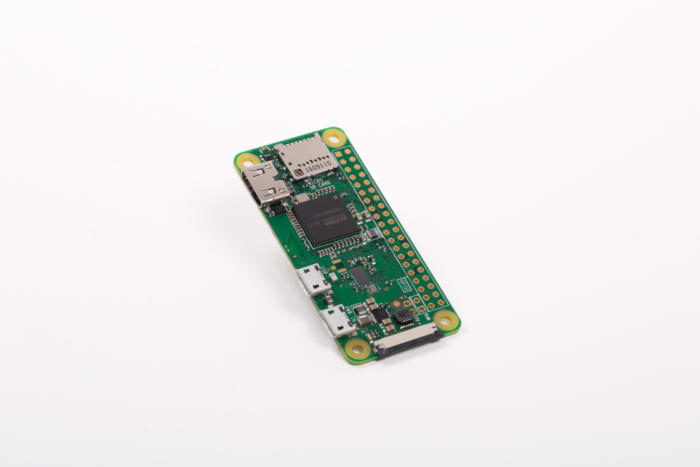
\includegraphics[width=\textwidth,height=\textheight,keepaspectratio]{rpizerow.jpg}
			\caption{Το Raspberry Pi Zero W.}
		\end{figure}

		Στην "καρδιά" του RPi Zero W υπάρχει ένας Broadcom BCM2835, 32-bit επεξεργαστής αρχιτεκτονικής ARMv6, χρονισμένος στο 1Ghz. Για μνήμη τυχαίας προσπέλασης χρησιμοποιούνται 512MB Low Power Double Data Rate 2 (LPDDR2) RAM. Πανω στο RPi Zero W δεν υπάρχει αποθηκευτικός χώρος, οπότε χρησιμοποιείται μια κάρτα MicroSD. 

		Ένα από τα σημαντικότερα σημεία ενός RPi Zero W είναι οι \textbf{\idxa{Δέκτες Εισόδου/Εξόδου Γενικού Σκοπού (General Purpose Input/Output, GPIO)}}. Μέσω αυτών καθίσταται δυνατόν να συνδεθεί το RPi με μια πληθώρα εξωτερικών αισθητήρων, διακοπτών (Relay Modules), πλακετών επέκτασης (γνωστά ως HATs), και εξαρτημάτων και να αντλήσει πληροφορίες από αυτά ή να τα ελέγξει.

	\subsection{Relay Module}
		\label{sub:relay}
		Προκειμένου να μπορέσει να συνδεθεί το RPi με το ήδη υπάρχον σύστημα ξεκλειδώματος, χρειάζεται ένας ηλεκτρονικά ελεγχόμενος διακόπτης. Θα χρησιμοποιηθεί ένα \textbf{\idxa{Relay Module}}. Τα Relay Modules χρησιμοποιούνται ως διακόπτες προκειμένου να ελέγχονται κυκλώματα μέσω υπολογιστών/μικροελεγκτών, οι οποίοι λειτουργούν μέσω σημάτων μικρής ισχύος\sucite{relay_purpose}.

		Τα Relay Modules κυκλοφορούν σε πολλούς τύπους. Οι τρείς κυριότεροι είναι:
		\begin{itemize}
			\item 5V Compatible, Active Low. 
			\item 5V/3.3V Compatible, Active High.
			\item 3.3V Compatible Active High/Low.
		\end{itemize}

		Το Raspberry Pi, εφόσον λειτουργεί σε λογική 3.3V, είναι συμβατό με τους 2 τελευτέους τύπους. Αν θελήσει ο χρήστης να χρησιμοποιήσει ένα Relay Module που να λειτουργεί σε λογική 5V και είναι Active Low, θα χρειαστεί να χρησιμοποιήσει ένα Arduino.

		Τα Relay Modules αποτελούνται από ένα Relay τύπου SRD, έναν φωτοσυζευκτή (Optocoupler), ευθύνη του οποίου είναι να απομονώνει το κύκλωμα ωστε να μην επηρρεάσει η υψηλή τάση (σε περίπτωση που χρησιμοποιείται από το σύστημα ξεκλειδώματος του κτηρίου) το υπόλοιπο κύκλωμα, ένα Transistor και μια δίοδο. Είναι σημαντικό να τονιστεί οτι καλό είναι να μην χρησιμοποιούνται Relay Modules που δεν φέρουν Φωτοσυζευκτή, καθώς μπορεί, σε περίπτωση που χρησιμοποιείται υψηλή τάση, να επηρρεαστεί, ακόμα και να καεί, το Raspberry Pi ή/και το Arduino. %TODO Needs citation.

		%TODO Add Figure...

	\subsection{Arduino UNO}
		Το \textbf{\idxa{Arduino UNO}} είναι ένας Ανοικτού-Κώδικα (Open Source) μικροελεγκτής σχεδιασμένος από την \href{https://www.arduino.cc/}{Arduino.cc}. Είναι βασισμένος πάνω στον ATmega328 microcontroller της Atmel. Μπορεί να χρησιμοποιηθεί προκειμένου να χειρίζεται και να αντλεί πληροφορίες από διάφορα εξαρτήματα στον φυσικό κόσμο. Εξαιτίας της μεγάλης ευελιξίας του έχει γίνει μία από τις δημοφιλέστερες επιλογές για κατασκευαστές, οι οποίοι το χρησιμοποιούν για μια τεράστια γκάμα εφαρμογών\sucite{arduino_definition}.

		To Arduino UNO μπορεί να χρησιμοποιηθεί σε περίπτωση που δεν χρησιμοποιηθεί κάποιο Relay συμβατό με το Raspberry Pi (βλ. \fullref{sub:relay}), αρκεί να λειτουργεί με λογική 5V.

		Μπορεί, έναντι του Arduino UNO, και προκειμένου να εξοικονομηθεί χώρος, να χρησιμοποιηθεί ένα \idxa{Arduino Nano}, το οποίο έχει όλες τις αναγκαίες λειτουργίες για την λειτουργία του PiLock.

		Ρεύμα για την λειτουργία του Arduino παρέχεται από την θύρα Micro USB του RPi, και μέσω αυτού δίνεται ρεύμα και σε οποιοδήποτε Relay Module συνδεθεί με αυτό. Για να γίνει αποστολή δεδομένων από το RPi στο Arduino χρησιμοποιείται η \idxa{Σειριακή Θύρα (Serial Port)} του Arduino.

		\begin{figure}[h]
			\centering
				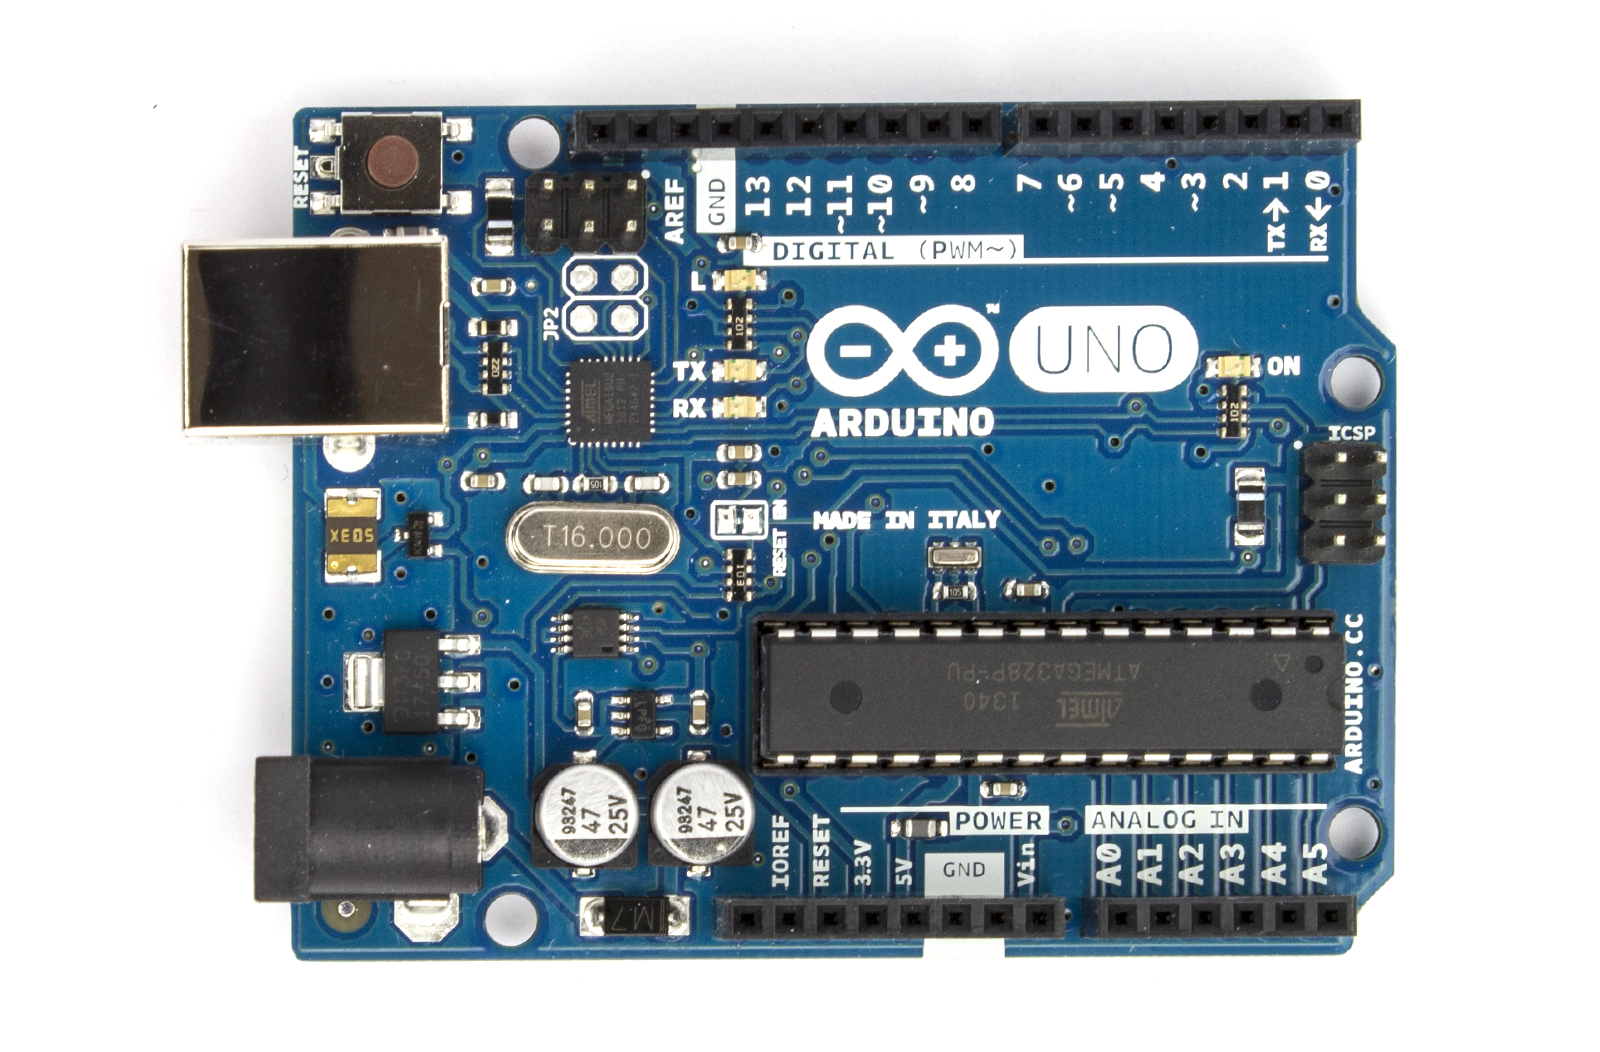
\includegraphics[width=0.5\textwidth,height=0.5\textheight,keepaspectratio]{arduino_uno.jpg}
			\caption{Arduino Uno Rev3, oomlout (2015), Flickr, CC BY-SA 2.0}
		\end{figure}

	\subsection{Λοιπό Hardware}
		Προκειμένου να συναρμολογηθεί η κατασκευή θα χρειαστουν κάποια συγκεκριμένα υλικά, εύκολα προμηθεύσιμα από διάφορα μαγαζιά πώλησης υλικών για ηλεκτρονικές κατασκευές.

		\subsubsection{Κουτί Κατασκευής (Project Box):}
			Ανάλογα τον τρόπο σύνδεσης που θα χρησιμοποιηθεί για την σύνδεση του RPi με το Relay Module, και ανάλογα με το αν είναι συμβατό το Relay Module με λογική 3.3V, θα χρειαστεί διαφορετικό μέγεθος κουτιού κατασκευής. 

			\paragraph{Σύνδεση χωρίς χρήση Arduino:}
				Ο προεπιλεγμένος τρόπος σύνδεσης, από την έκδοση \verb|0.3.1| και μετά είναι χωρίς την χρήση Arduino. Έπειτα από μετρήσεις βρέθηκε οτι το κατάλληλο κουτί κατασκευής έχει διαστάσεις 10cm x 10cm.
			\paragraph{Σύνδεση με Arduino:}
				Εφόσον χρειάζεται να γίνει σύνδεση με Arduino (προκειμένου να μπορεί να λειτουργήσει το Relay Module), έπειτα απο μετρήσεις βρέθηκε οτι το κατάλληλο κουτί κατασκευής έχει διαστάσεις 18cm x 14cm.

		\subsubsection{Καλώδια σύνδεσης:}
			Για να συνδεθεί το Relay Module με το RPi (ή το Arduino), θα χρειαστούν κάποια συγκεκριμένα καλώδια σύνδεσης γνωστά ως Jumper Wires. Τα Jumper Wires κάνουν εύκολη την σύνδεση σε διάφορα εξαρτήματα καθώς δεν χρειάζονται συγκόλληση \textsuperscript{\cite{jumper_wires}}.

		 	\paragraph{Σύνδεση χωρίς χρήση Arduino:}
		 		Θα χρειαστούν τουλάχιστον 3 Jumper Wires Female-Male (ή Female-Female, σε περίπτωση χρήσης του Male Header).
		 	\paragraph{Σύνδεση με Arduino:}
		 		\label{par:ard_conn}
		 		Θα χρειαστούν τουλάχιστον 3 Jumer Wires Female-Male, αν χρησιμοποιηθεί Arduino UNO ή 3 τουλάχιστον καλώδια Female-Female, αν χρησιμοποιηθεί Arduino Nano. Επίσης, θα χρειαστεί ένα καλώδιο Micro USB-B to USB-A (\idxa{OTG Cable}) και ένα καλώδιο USB-A to USB-B αν χρησιμοποιηθεί ένα Arduino UNO ή ένα καλώδιο USB-A to Micro USB-B σε περίπτωση χρήσης Arduino Nano.

		 	\begin{figure}[h]
			\centering
				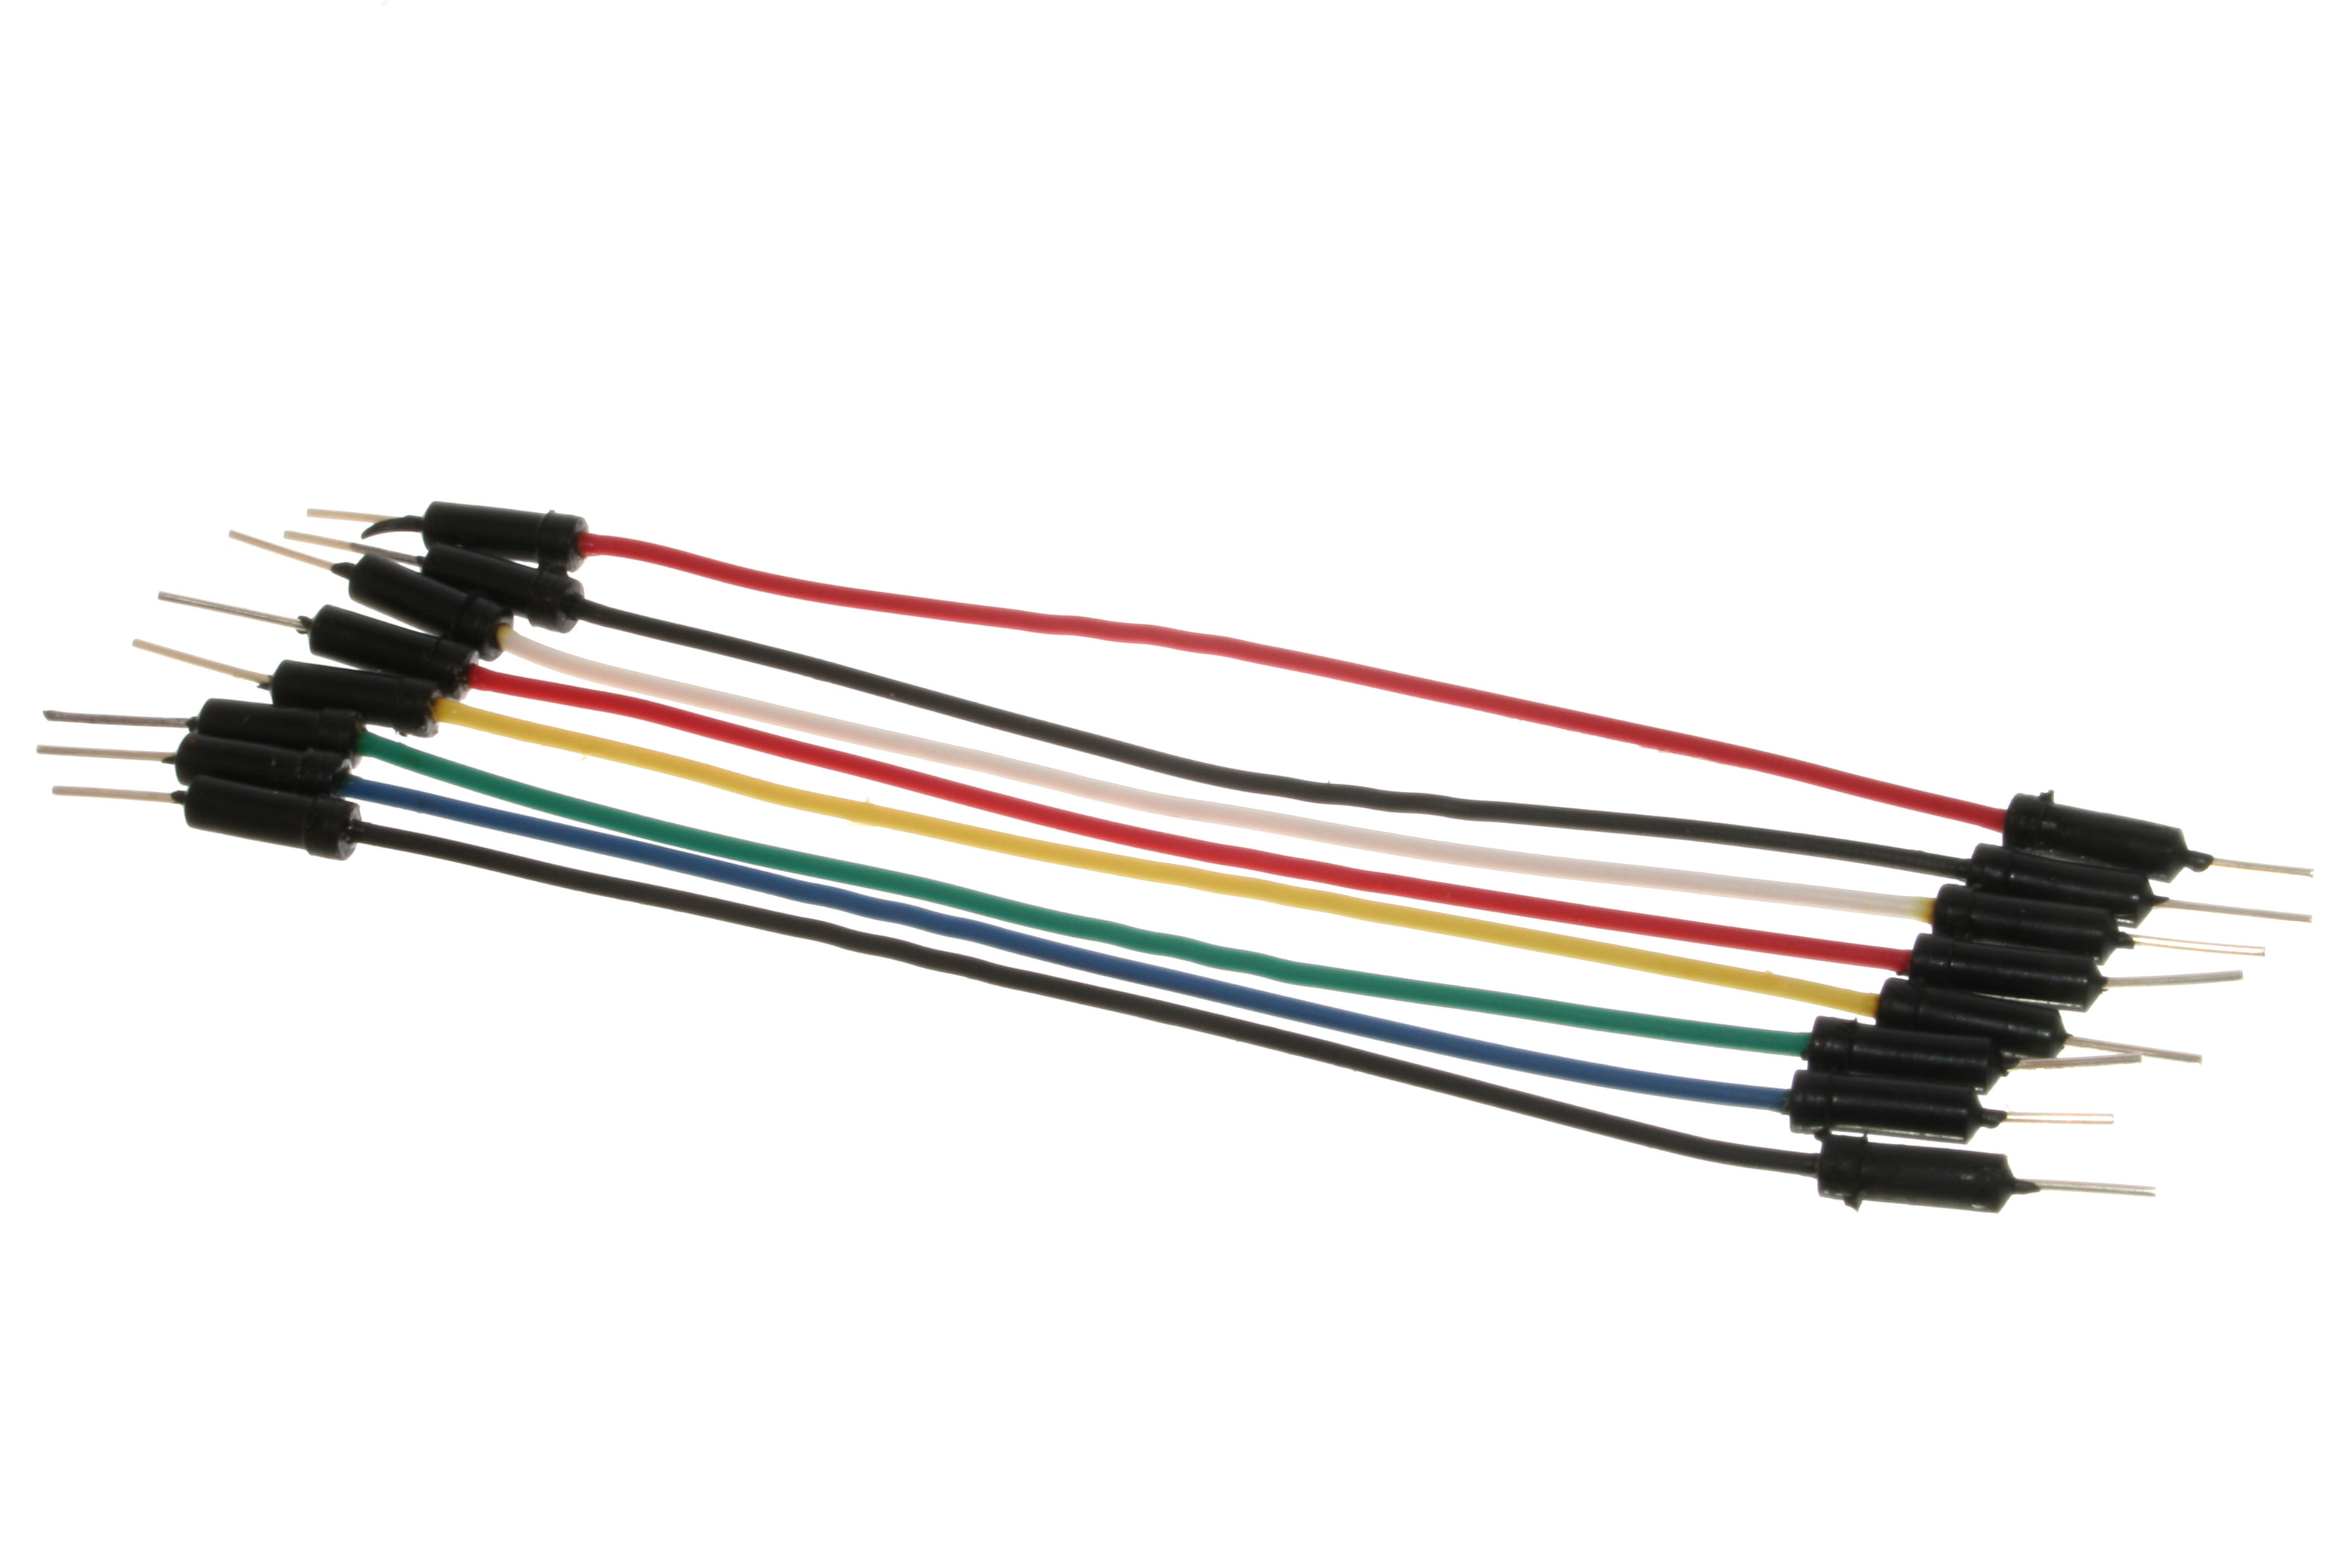
\includegraphics[width=0.5\textwidth,height=0.5\textheight,keepaspectratio]{jumper_wires.jpg}
				\caption{Jumper Wires (Male-Male), oomlout (2009), Flickr, CC BY-SA 2.0}
			\end{figure}

\section{Κόστος Κατασκευής του PiLock}
	Με βάση την παραπάνω λίστα υλικών που θα χρησιμοποιηθούν για την συναρμολόγηση του PiLock, μπορεί να εξαχθεί ένα τελικό κόστος για την προμήθεια των υλικών αυτών. Να σημειωθεί οτι η εξαγωγή των τιμών αυτών έγινε έπειτα από έρευνα σε διάφορα ηλεκτρονικά μαγαζιά, είτε Ελληνικά, είτε του εξωτερικού, προκειμένου να κρατηθεί σε όσο το δυνατόν χαμηλότερα πλαίσια το τελικό κόστος.

	\begin{center}
	\begin{tabular}{||c c||}
		\hline
		Υλικό & Κόστος \\ [0.5ex] 
		\hline\hline
		Raspberry Pi Zero W\textsuperscript{*} & 17.46\euro \\
		Project Box (18x14) & 4.90\euro \\
		Relay Module & 2.75\euro \\
		Arduino Uno (Κλώνος) & 5.00\euro \\
		Καλώδια & 0.70\euro \\
		\hline\hline
		Τελικό Κόστος: & 30.81\euro \\
		\hline
	\end{tabular}
	\end{center}

	{\footnotesize *: Συμπεριλαμβάνεται Καλώδιο OTG, GPIO Headers}

	Να σημειωθεί οτι, όπως είναι αντιληπτό, στο παραπάνω κόστος συμπεριλαμβάνεται και το Arduino. Εάν αγοραστεί συμβατό με το Raspberry Pi, Relay Module, το κόστος κατεβαίνει στα 23,81\euro, καθώς δεν απαιτείται η χρήση Arduino και, κατ'επέκταση, απαιτείται και μικρότερο Project Box.

    \chapter{Συστήματα Ελέγχου Πρόσβασης Πολυκατοικιών/Σπιτιών}
    \label{ch:unlock_mechanism}
Πριν να εξηγήσουμε τον τρόπο κατασκευής και λειτουργίας του PiLock, είναι αναγκαίο να αναφερθούμε στον τρόπο λειτουργίας των περισσότερων κλειδαριών σπιτιών, πολυκατοικιών ή και γραφείων.

Το σύστημα ξεκλειδώματος που χρησιμοποιείται στις περισσότερες κατοικίες αποτελείται από 2 εντελός ξεχωριστά και ανεξάρτητα συστήματα: Το σύστημα του θυροτηλεφώνου, δηλαδή το σύστημα μέσω του οποίου γίνεται η αναγνώριση του επισκέπτη (μέσω φωνής ή/και εικόνας), και το σύστημα ενεργοποίησης της κλειδαριάς. Στην παρούσα διατριβή θα αναφερθούμε αποκλειστικά στο δεύτερο σύστημα.

Οι ηλεκτρικές κλειδαριές που χρησιμοποιούνται σε πολυκατοικίες συνήθως αποτελούνται από ένα μάνταλο το οποίο, όταν το σύστημα ενεργοποιηθεί μέσω ρεύματος, απελευθερώνεται με αποτέλεσμα να μπορεί ελεύθερα η πόρτα να ανοίξει.

\begin{figure}[h]
	\centering
		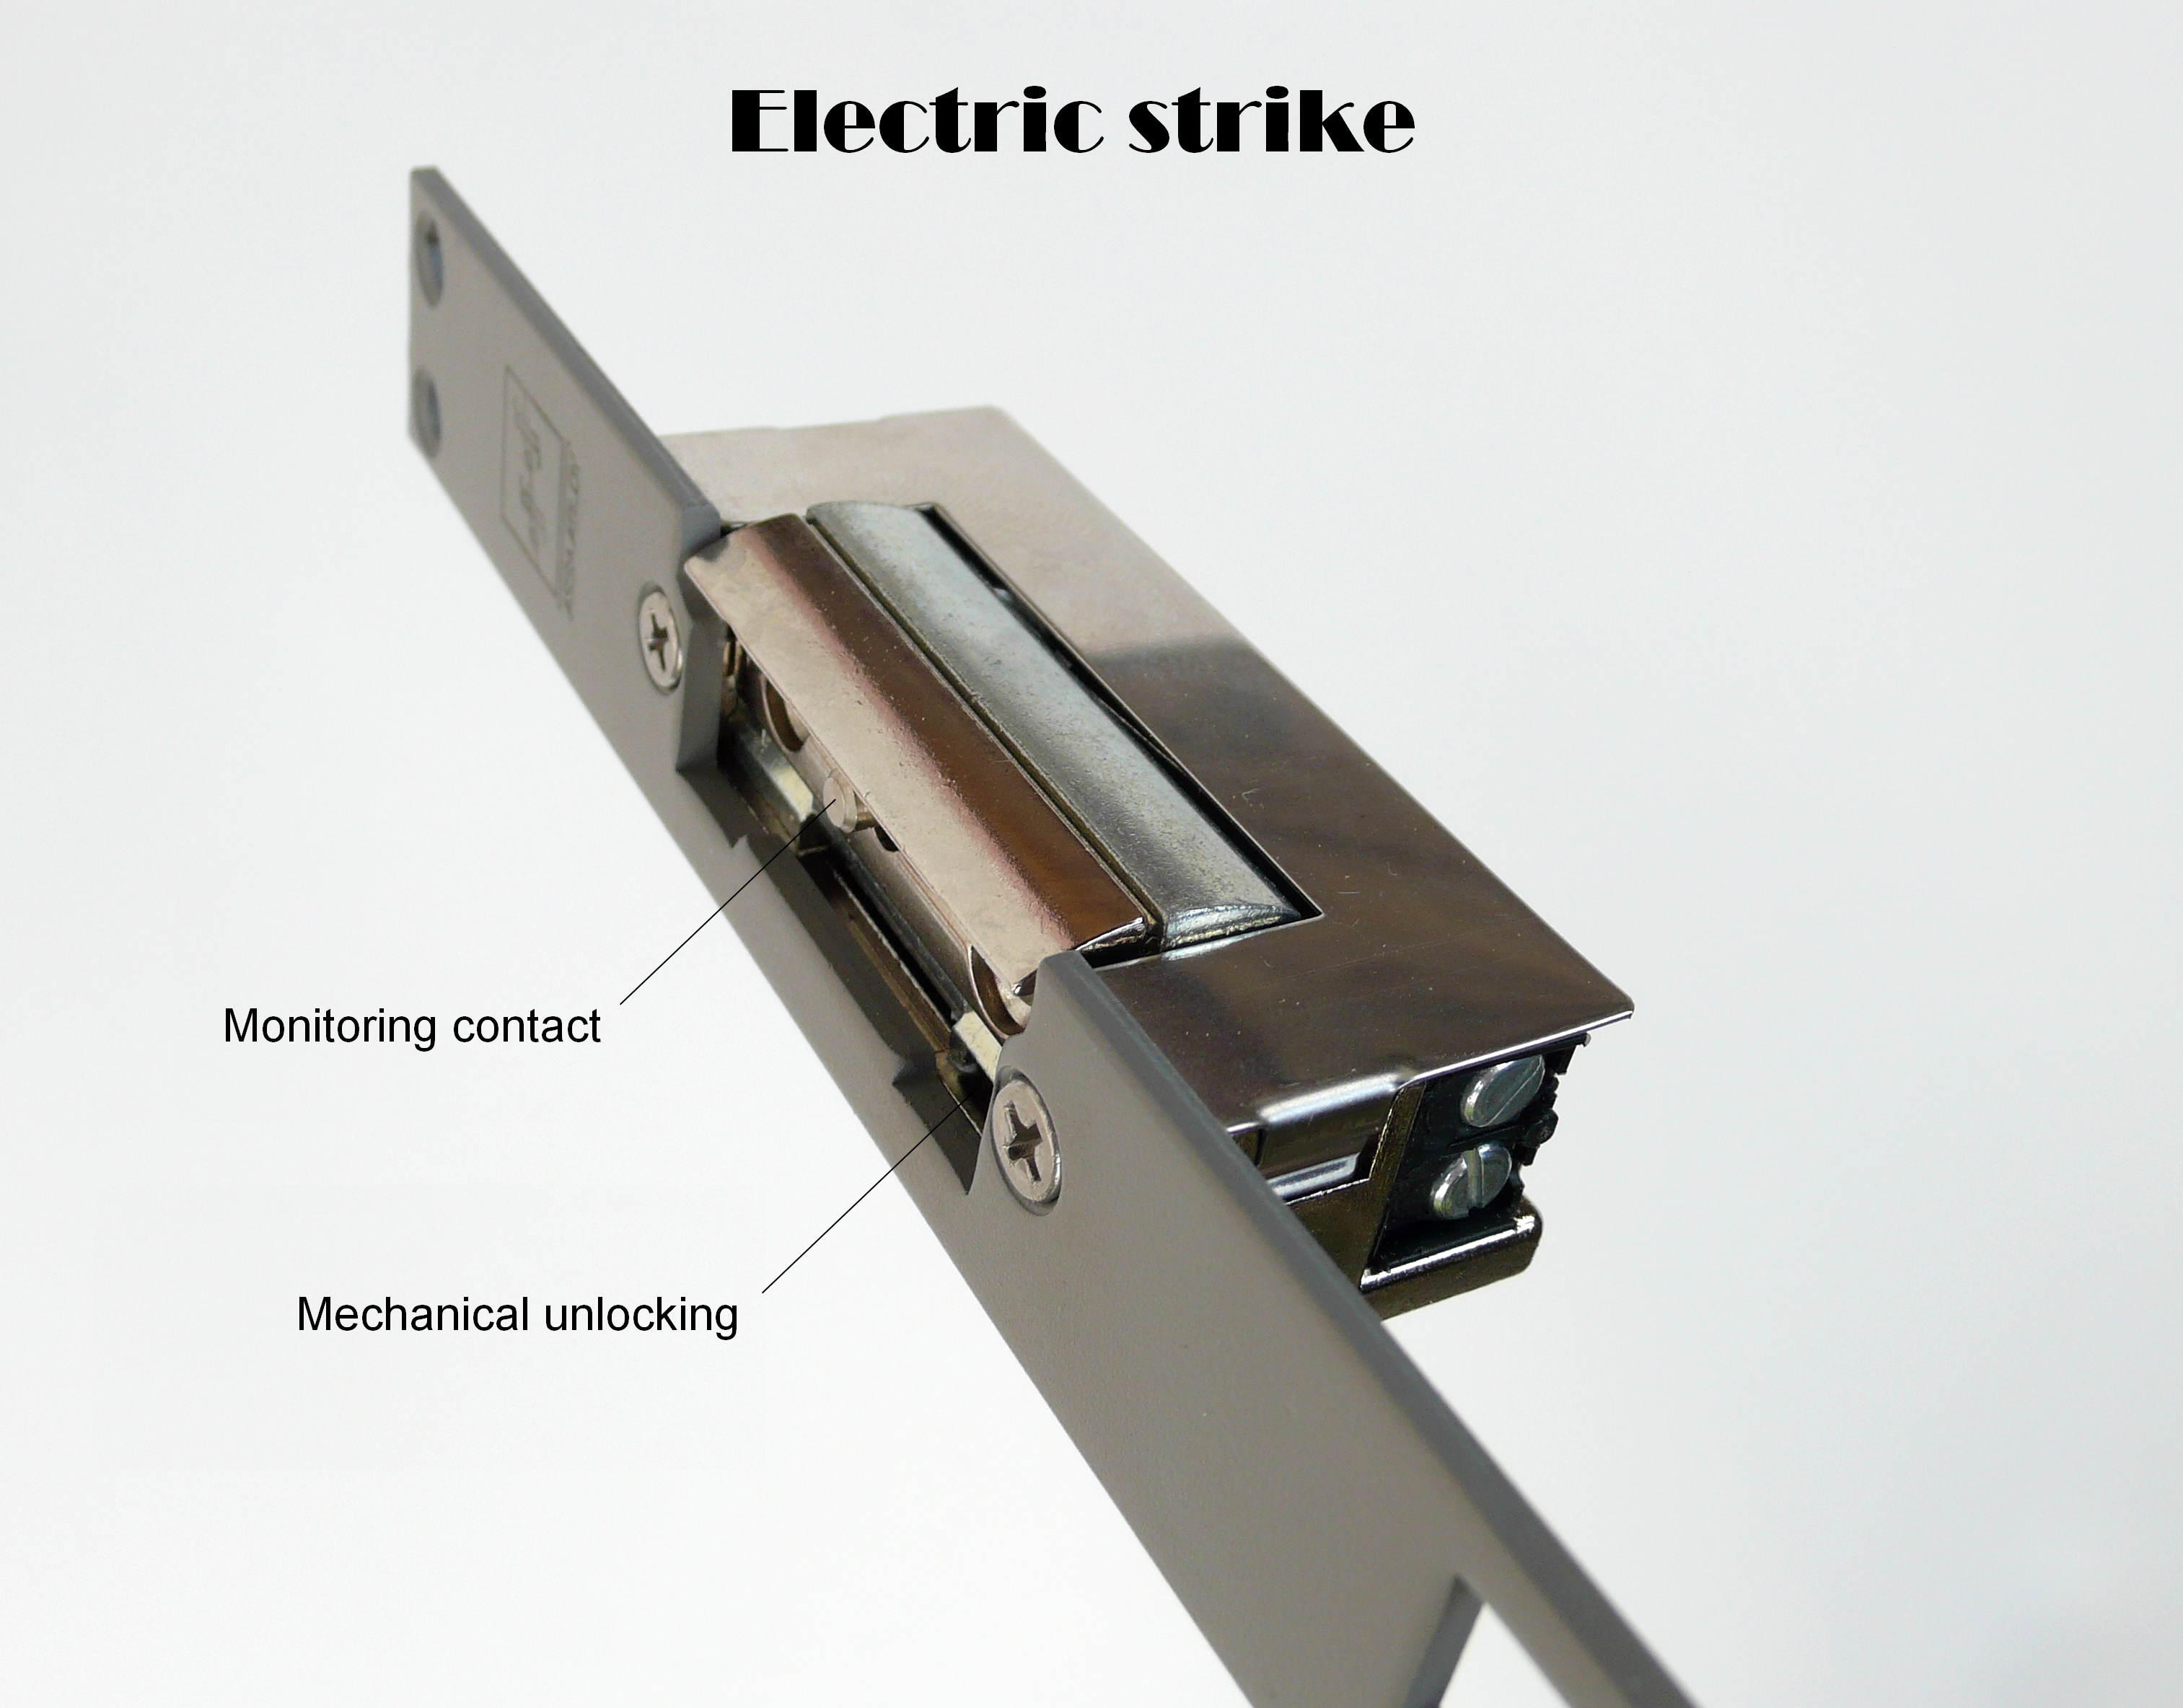
\includegraphics[width=0.5\textwidth,height=0.5\textheight,keepaspectratio]{Electric_strike.jpg}
	\caption{Ηλεκτρική κλειδαριά πολυκατοικίας με σύστημα καταγραφής κατάστασης κλειδώματος}
\end{figure}

Η ενεργοποίηση του παραπάνω συστήματος γίνεται μέσω ενός διακόπτη αναρτημένου πάνω στο θυροτηλέφωνο του κάθε διαμερίσματος. Η τροφοδοσία των συστημάτων αυτών μπορεί να γίνεται είτε μέσω απευθείας τροφοδοσίας από το ηλεκτρικό δίκτυο, είτε μέσω κάποιου μετασχηματιστή σε χαμηλότερες τάσεις.

Προκεικένου να μπορέσουμε να ελέγξουμε το σύστημα ξεκλειδώματος, θα πρέπει να μπορέσουμε να βάλουμε έναν δεύτερο διακόπτη, να λειτουργεί παράλληλα με τον πρώτο.  %TODO Refer to next chapter.

Για να γίνει αυτό, θα πρέπει να εντοπιστεί το κύκλωμα που συνδέεται με τον ήδη υπάρχοντα διακόπτη ξεκλειδώματος (του θυροτηλεφώνου) και να τοποθετηθούν 2 καλώδια σε παράλληλη σύνδεση με τον ήδη υπάρχοντα διακόπτη.

Για τον εντοπισμό θα πρέπει να αποσυνδεθεί ο διακόπτης από τον τοίχο, λύνοντας τις βίδες οι οποίες τον συγκρατούν. Προκειμένου να γίνει υπο ασφαλές συνθήκες, συνίσταται να απενεργοποιηθεί η παροχή ρεύματος στο παρόν τμήμα της οικίας, μέχρι να ολοκληρωθεί η εγκατάσταση. Αυτό μπορεί να γίνει είτε κατεβάζοντας την ασφάλεια που αντοιστοιχεί στο συγκεκριμένο τμήμα της κατοικίας, από τον ηλεκτρικό πίνακα, είτε απενεργοποιόντας τον γενικό διακόπτη τροφοδοσίας της κατοικίας.

Η τελική εγκατάσταση θα υπογραμμιστεί σε επόμενο κεφάλαιο.

    \chapter{Νέος μηχανισμός ξεκλειδόματος}
    Στο προηγούμενο κεφάλαιο είδαμε από τι αποτελείται ένα σύνηθες σύστημα ξεκλειδώματος πόρτας πολυκατοικίας/σπιτιού. Στο παρόν κεφάλαιο θα αναλύσουμε τον τρόπο σύνδεσης των εξαρτημάτων (βλ \fullref{sec:hardw}), και τον προγραμματισμό τους ώστε να μπορεί να πυροδοτηθεί ξεκλείδωμα της πόρτας μέσω υπολογιστή.

\section{Προετοιμασία του Raspberry Pi}
	Πρώτο βήμα πριν να γίνει η οποιαδήποτε σύνδεση μεταξύ εξαρτημάτων είναι αναγκαίο να γίνει η εγκατάσταση της τελευταίας έκδοσης του Raspbian Lite στο Raspberry Pi Zero W, καθώς επίσης και να συνδεθεί με το internet. Χρησιμοποιείται η έκδοση Lite έναντι της πλήρης έκδοσης, καθώς δεν χρειάζεται γραφικό περιβάλλον όπως επίσης και τα περισσότερα πακέτα που υπάρχουν προεγκατεστημένα στην πλήρη έκδοση.

	Αφότου γίνει η εγκατάσταση του λειτουργικού συστήματος στην κάρτα MicroSD, μπορεί να γίνει η σύνδεση στο Internet είτε Headlessly (χωρίς, δηλαδή, να χρειαστεί να συνδεθεί οθόνη στο RPi), βάζοντας το αρχείο στο \verb|boot| partition (διαμέρισμα) της κάρτας μνήμης, και εφαρμόζοντας το παρακάτω configuration, μέσα στο αρχείο \verb|wpa_supplicant.conf|\textsuperscript{\cite{rpi_wifi_headless}}:

	\begin{lstlisting}
	network={
		ssid="YOUR_NETWORK_NAME"
		psk="YOUR_PASSWORD"
	}\end{lstlisting} 

	Στο πεδίο \verb|ssid| πρέπει να μπει το όνομα του δικτύου στο οποίο πρόκειται να συνδεθεί το RPi. Στο πεδίο PSK πρέπει να γίνει τοποθέτηση του κλειδιού πρόσβασης του δικτύου. Σε περίπτωση που δεν χρησιμοποιείται κρυπτογραφία στο δίκτυο (δεν προτείνεται καθώς μπορεί να συμβεί υποκλοπή δεδομένων από τρίτους), μπορούμε να εισάγουμε το παρακάτω configuration στο ίδιο αρχείο:

	\begin{lstlisting}
	network={
		ssid="YOUR_NETWORK_NAME"
		key_mgmt=NONE
	}\end{lstlisting} 

	Τέλος, πρέπει να γίνει ενεργοποίηση του SSH Daemon στο Raspbian, προκειμένου να είναι εφικτή η απομακρυσμένη σύνδεση στο RPi, μέσω τοπικού δικτύου. Λόγω κατασκευής δικτύων bot (botnets) από διάφορους κακόβουλους χρήστες προκειμένου να γίνουν επιθέσεις DDOS (Distributed Denial of Service) από συσκευές Internet of Things που χρησιμοποιούν τα προεπιλεγμένα (default) στοιχεία πρόσβασης (Username, Password), προς διάφορους στόχους, από τον Νοέμβριο του 2016 είναι απενεργοποιημένος εξ' αρχής ο SSH Daemon και πρέπει να ενεργοποιηθεί από τον χρήστη, αν τον χρειάζεται \textsuperscript{\cite{raspbian_nov2016_upd}}. Για να γίνει αυτό, πρέπει να δημιουργηθεί ένα άδειο αρχείο με το όνομα \verb|ssh| μέσα στο \verb|boot| partition της κάρτας μνήμης του RPi.

	Αφότου γίνει η πρώτη εκκίνηση του RPi και βεβαιωθεί οτι υπάρχει ενεργή σύνδεση στο διαδίκτυο, πρέπει να γίνει σύνδεση στο Raspberry Pi μέσω SSH (Username: pi, Password: raspberry)\textsuperscript{\cite{default_creds}} και να γίνουν τα ακόλουθα βήματα, προκειμένου να ενημερωθεί πλήρως το Raspbian:

	\subsection{Αλλαγή των προεπιλεγμένων στοιχείων πρόσβασης}
		Όπως αναφέραμε προηγουμένως, προκειμένου να μην υπάρξει στο μέλλον κίνδυνος επίθεσης, πρέπει να γίνει αλλαγή των προεπιλεγμένων στοιχείων πρόσβασης στο Raspbian. Πρέπει να εκτελεστεί η εντολή \verb|passwd|, και να γίνει εισαγωγή ενός νέου κωδικού πρόσβασης. Ο νέος κωδικός, προκειμένου να είναι ασφαλής, πρέπει να αποτελείται από τουλάχιστον 12 χαρακτήρες, να μην περιέχει μέσα ονόματα, ονόματα από μέρη, ή γενικά λέξεις οι οποίες υπάρχουν μέσα σε λεξικά, και τέλος θα πρέπει να περιέχει πεζά γράμματα, κεφαλαία, αριθμούς, και σύμβολα\textsuperscript{\cite{secure_passwords}}.

	\subsection{Ενημέρωση του Raspbian}
		Προκειμένου να εξασφαλιστεί η βέλτιστη λειτουργία και η μέγιστη ασφάλεια στο σύστημα, χρειάζεται να γίνει ενημέρωση των πακέτων του λειτουργικού συστήματος. Πρέπει να γίνει εκτέλεση των επόμενων 2 εντολών\textsuperscript{\cite{raspbian_update}}:

		\begin{lstlisting}[language=bash]
		sudo apt-get update
		sudo apt-get dist-upgrade\end{lstlisting}

	Αφότου γίνει η αλλαγή των προεπιλεγμένων στοιχείων πρόσβασης και η ενημέρωση του συστήματος, πρέπει να απενεργοποιηθεί το σύστημα προκειμένου να συνδεθεί με το Relay. 

\section{Σύνδεση με το Relay}
	Για να γίνει η σύνδεση του Raspberry Pi με το Relay, πρέπει να επιλέξουμε έναν από τους 2 τρόπους σύνδεσης, ανάλογα με το τι Relay Module θα χρησιμοποιηθεί (βλ. \fullref{sub:relay}).

	\subsection{Σύνδεση χωρίς την χρήση Arduino}
		Προκειμένου να γίνει σύνδεση του RPi με το Relay Module, θα χρειαστεί να κολληθούν κεφαλές υποδοχής για Jumper Wires στα GPIO του Raspberry Pi. Μπορούν να χρησιμοποιηθούν είτε Female, είτε Male τύπου Headers, αλλά από αυτό θα εξαρτηθεί τι Jumper Wires θα χρειαστούν για να συνδεθεί το RPi με το Relay Module (Male-Female αν χρησιμοποιηθεί Female Header, Female-Female αν χρησιμοποιηθεί Male Header).

		\begin{figure}[h]
			\centering
				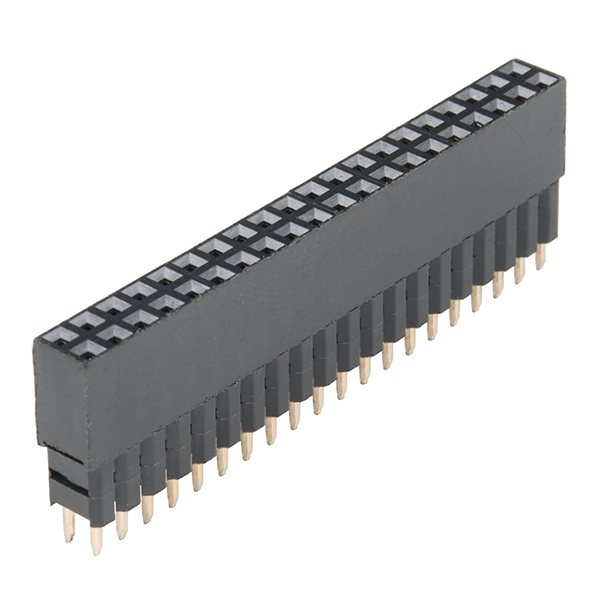
\includegraphics[width=0.5\textwidth,height=0.5\textheight,keepaspectratio]{female_gpio_headers.jpg}
			\caption{Female GPIO Headers, SparkFun Electronics (2016), Flickr, CC-BY 2.0}
			\label{fig:headers}
		\end{figure}

		Αφότου γίνει η κόλληση των Headers, μπορούν να χρησιμοποιηθούν τα αντίστοιχα καλώδια προκειμένου να συνδεθεί το Relay Module. Πρέπει ο χρήστης που θα το συνδέσει να συμβουλευτεί το διάγραμμα των GPIO Pins (γνωστό ως Pinout). Στο συγκεκριμένο παράδειγμα (\imgref{fig:rpi_to_relay}), έχει συνδεθεί στο GPIO Pin 18 (πράσινο καλώδιο). Για παροχή ρεύματος χρησιμοποιείται το 3V3 Pin (κόκκινο καλώδιο) και για Ground χρησιμοποιείται ένα από όλα τα GND Pins (μαύρο καλώδιο).

		\begin{figure}[h]
			\centering
				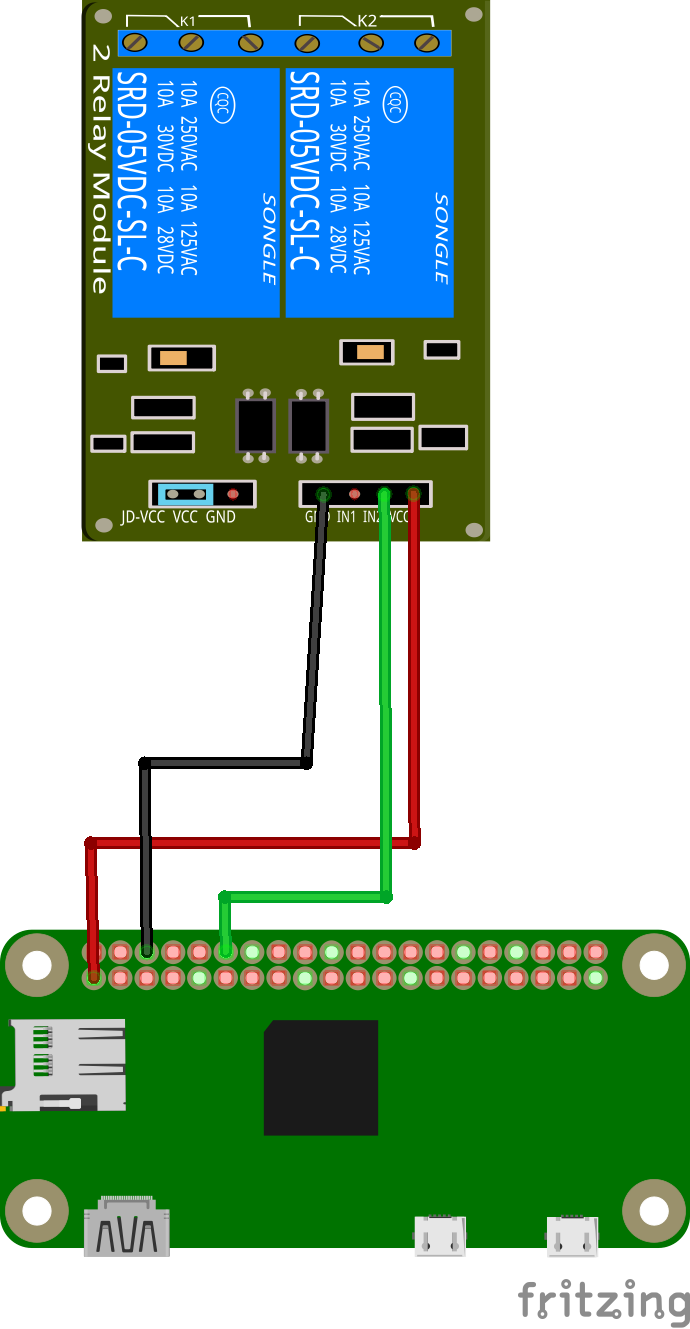
\includegraphics[width=0.5\textwidth,height=0.5\textheight,keepaspectratio]{rpi_to_relay.png}
			\caption{Σύνδεση ενός Raspberry Pi Zero W με ένα Relay Module}
			\label{fig:rpi_to_relay}
		\end{figure}


	\subsection{Σύνδεση με την χρήση Arduino}
		Αφότου γίνει Upload το Arduino Script που χρειάζεται για την λειτουργία του PiLock (βλ \fullref{sec:arduino_script}), μπορεί να γίνει σύνδεση του Arduino με το Relay. Το Relay Board μπορεί να συνδεθεί σε ένα από όλα τα Digital Pins του Arduino (πράσινο καλώδιο). Ρεύμα δίνεται μέσω του 5V Power Pin του Arduino και το Ground συνδέεται σε ένα εκ των τριών GND Pins του Arduino.

    \chapter{Προγραμματιστικό Περιβάλλον - Τεχνολογίες που Χρησιμοποιήθηκαν}
    Στο παρόν κεφάλαιο θα αναφερθούν και θα αναλυθούν τα εργαλεία που χρησιμοποιήθηκαν κατά την ανάπτυξη του PiLock, καθώς επίσης και στην διαχείρηση του έργου ανάπτυξης.

\section{Η σημασία χρήσης δωρεάν λογισμικού ανοικτού κώδικα κατά την ανάπτυξη του PiLock}
	Ως "Λογισμικό Ανοικτού Κώδικα" (Open Source Software) ορίζεται το λογισμικό του οποίου ο πηγαίος κώδικας είναι διαθέσιμος ελεύθερα προς το κοινό προκειμένου να μπορεί να τροποποιηθεί, να αναβαθμιστεί ή να μελετηθεί. Ο πηγαίος κώδικας, για τον απλό χρήστη είναι ένα τμήμα του λογισμικού που δεν έχει δει ποτέ. Σε έργα ανοικτού κώδικα, μπορεί ο οποιοσδήποτε να προτείνει διορθώσεις, αναβαθμίσεις ή προσθήκη χαρακτηριστικών\textsuperscript{\cite{FOSS_def}}. 

	Εξαιτίας αυτού του χαρακτηριστικού, και των αδειών που το υποστηρίζουν, το λογισμικό ανοικτού κώδικα μπορεί να χρησιμοποιηθεί για οποιοδήποτε σκοπό επιθυμεί ο χρήστης, χωρίς να περιορίζεται από κάποια άδεια χρήσης. Επίσης, παρέχει αυξημένη ασφάλεια, εφόσον μπορεί να δοκιμαστεί και να μελετηθεί από τους προγραμματιστές ο πηγαίος κώδικάς του. Στο λογισμικό κλειστού κώδικα, είναι αδύνατον να μελετηθεί και να τροποποιηθεί από τρίτους ο κώδικάς του, και κατ' επέκταση, εφόσον υπάρξει ένα κενό ασφαλείας θα πάρει συνήθως αρκετά περισσότερο χρόνο μέχρι να κυκλοφορήσει μια ενημέρωση ασφάλειας. Τέλος, εξαιτίας της ευελιξίας που παρέχει, το λογισμικό ανοικτού κώδικα μπορεί να τροποποιηθεί προκειμένου να μπορέσει καλύτερα να καλύψει τις ανάγκες του χρήστη\textsuperscript{\cite{FOSS_def}, \cite{FOSS_benefits}}.

	Μία υποκατηγορία του λογισμικού ανοικτού κώδικα είναι το \textbf{Δωρεάν Λογισμικό Ανοικτού Κώδικα (Free and Open Source Software, FOSS)}, το οποίο επιτρέπει στον χρήστη να το κατεβάσει και να το χρησιμοποιήσει χωρίς κάποιο κόστος. Το λογισμικό που χρησιμοποιήθηκε για την ανάπτυξη του PiLock ανήκει στην κατηγορία αυτή.

\section{Διαχείρηση του έργου}

	\subsection{Version Control}
		\label{subsec:vc}
		Καθ' όλη την διαδικασία ανάπτυξης του PiLock χρησιμοποιήθηκε σύστημα Version Control. Τα Συστήματα Version Control βοηθούν τον/τους προγραμματιστή/ές καθώς προσδίδουν ασφάλεια και ευελιξία κατά την ανάπτυξη και την συντήρηση ενός έργου. To \idxa{Git} είναι το λογισμικό Version Control που χρησιμοποιήθηκε κατά την ανάπτυξη του PiLock.

		Το Git δημιουργήθηκε από τον Linus Torvalds το 2005 προκειμένου να τον βοηθήσει στην ανάπτυξη του Linux Kernel\textsuperscript{\cite{Git_History}}. Διάφοροι άλλοι συνεισφέροντες προς το Linux Kernel βοήθησαν στην ανάπτυξη του Git, κατά την πρώτη περίοδο της ανάπτυξής του. Αποτελεί δωρεάν λογισμικό ανοικτού κώδικα και διανείμεται υπό την άδεια GNU General Public Licence, έκδοση 2\textsuperscript{\cite{Git_Licence}}. 

		Πιο συγκεκριμένα, εξαιτίας της ικανότητάς του Git να διατηρεί ιστορικό για όλα τα αρχεία ενός έργου, το έργο μπορεί να επανέλθει σε μία προηγούμενη κατάστασή του, ανά πάσα στιγμή. Οι "καταστάσεις" είναι γνωστές ως "\idxa{Commits}". Με αυτό τον τρόπο, δεν απορρίπτεται κώδικας, πολλές φορές πολύτιμος για την ανάπτυξη ενός έργου. Μέσω των commits, μπορεί κάποιος να βεβαιωθεί ποιος έκανε αλλαγές στον κώδικα σε οποιοδήποτε σημείο επιθυμεί. Αξίζει να αναφερθεί η δυνατότητα της ψηφιακής υπογραφής των commits μέσω του \idxa{GNU Privacy Guard (GPG)}, προκειμένου να αποφευχθεί προσωποποίηση\textsuperscript{\cite{Git_commit_assurance}}. Επίσης, μέσω του συστήματος \idxa{Staging} του Git, ο προγραμματιστής γνωρίζει τι ακριβώς κρατείται σε ένα νέο Commit, όποτε καταχωρηθεί. Με το \idxa{Branching System} του Git, καθίσταται δυνατόν να τροποποιείται ή να προστίθεται κώδικας και νέα features χωρίς να τροποποιείται ο Stable κώδικας του έργου (για παράδειγμα, το κάθε release χρησιμοποιεί υποχρεωτικά νέο branch), ο οποίος "ενημερώνεται" στο τέλος του κάθε release/feature, προκειμένου να αποφευχθούν προβλήματα. Τέλος, το Git διευκολύνει σημαντικά την συνεργασία μεταξύ προγραμματιστών καθώς μπορεί ο κάθε προγραμματιστής να δουλεύει το δικό του "κομμάτι" κώδικα, χωρίς να επηρρεάζει την πρόοδο των υπολοίπων προγραμματιστών που δουλεύουν πάνω στο έργο.

		Στην ανάπτυξη του PiLock, το λογισμικό της πλευράς του Εξυπηρετητή, του Πελάτη καθώς επίσης και τα σενάρια ξεκλειδώματος (Unlock Scripts) διαχειρίζονται ξεχωριστά σε διαφορετικά αποθετήρια. Συγκεκριμένα, τα σενάρια ξεκλειδώματος αποτελούν Submodule του λογισμικού του εξυπηρετητή, δηλαδή μπορεί να εμφολευθεί ως ξεχωριστό αποθετήριο μέσα σε ένα ήδη υπάρχον αποθετήριο, ως κομμάτι του.

		Προκειμένου να γίνει σωστή διαχείρηση της διαδικασίας ανάπτυξης, ακολουθήθηκαν κάποιοι κανόνες. Οι κανόνες αυτοί διασφαλίζουν την ακαιρεότητα του κώδικα ανα πάσα στιγμή κατά την ανάπτυξη. Πιο συγκεκριμένα:

		\begin{itemize}
			\item Η σταθερή (Stable) έκδοση του κώδικα βρίσκεται στο master branch.
			\item Όποια αλλαγή πρόκειται να γίνει στον κώδικα, είτε αυτή είναι hotfix, είτε κάποιο νέο feature, είτε documentation, θα πρέπει να γίνεται αποκλειστικά σε νέο branch με χαρακτηριστικό τίτλο, ο οποίος να ξεκινά από το ανάλογο πρόθεμα (prefix). Συγκεκριμένα, αν πρόκειται για νέο feature να χρησιμοποιείται το "feature" prefix, αν πρόκειται για bugfix να χρησιμοποιείται το "bug" ή το "hotfix" prefix, και αν πρόκειται για αλλαγή στο documentation ή στο Readme, να χρησιμοποιείται το "doc" prefix. (Πχ. feature/pin\_changing)
			\item Τα νέα Branches, εφόσον ελεγχθούν, θα πρέπει να συγχωνεύονται στο αντίστοιχο branch στο οποίο απευθύνονται (βλ. παρακάτω).
			\item Νέα λειτουργικότητα (νέα features) προστίθεται μόνο στα νέα releases (στο branch του εκάστοτε νέου release). Τα hotfix καθώς επίσης και διάφορα bugs μπορούν να συγχωνεύονται απευθείας με το master, αρκεί να έχουν ελεγχθεί εξονυχιστικά πρώτα και να είναι υψηλής προτεραιότητας.
			\item Το master branch, καθώς επίσης και τα branches για νέα releases θα πρέπει να είναι κλειδωμένα και να δέχονται συγχονεύσεις μόνο εφόσον περάσει από έγκριση ο κώδικας μέσω κάποιου \idxa{Pull Request} ή \idxa{Merge Request}.
		\end{itemize} 

		Αρχικά, μέχρι την πρώτη δημόσια έκδοσή του (\verb|0.2.0|), ο κώδικας του PiLock φιλοξενούνταν στον προσωπικό εξυπηρετητή του δημιουργού, και τα αποθετήρια του διαχειρίζονταν μέσω του δωρεάν λογισμικού διαχείρησης αποθετηρίων Git γνωστό ως \idxa{GitLab} (\url{https://about.gitlab.com}). Αργότερα, από την πρώτη δημόσια έκδοσή του PiLock και μετά, ξεκίνησε να χρησιμοποιείται το \idxa{GitHub} (\url{https://github.com}) ως χώρος φιλοξενίας του έργου και των αποθετηρίων του.

	\subsection{Issue Tracking}
		Κατά την ανάπτυξη του PiLock, έγινε χρήση τόσο του συστήματος Issue Tracking του GitLab, όσο και του GitHub. Τα συστήματα \idxa{Issue Tracking}, χρησιμοποιούνται για να κρατάνε μια λίστα με διάφορα "ζητήματα" που προκύπτουν κατά την ανάπτυξη ενός έργου ή που προέρχονται από εξωτερικούς χρήστες. Στην 2η κατηγορία ανήκουν διάφορα αιτήματα νέας λειτουργικότητας, ή διάφορα bugs τα οποία μπορεί να έχουν αναφερθεί, κατά την χρήση του λογισμικού ή κατά την διάρκεια δοκιμών (testing). Issues επίσης μπορεί να προκύψουν από εξωτερικούς χρήστες ως απλά ερωτήματα για την χρήση του λογισμικού.

		Τα Issues, έχουν 2 κύριες καταστάσεις: Open (Ανοικτό), Closed (Κλειστό/Ολοκληρωμένο). Τα ανοικτά issues είναι τα αυτά που ακόμα δεν έχουν ικανοποιηθεί οι απαιτήσεις τους, ή είναι σε διαδικασία ανάπτυξης. Τα κλειστά issues είναι τα εκπληρωμένα issues ή όσα issues δεν είναι δυνατόν να εκπληρωθούν για κάποιο λόγο, και δεν πρόκειται να αναπτυχθούν άλλο.

		Προκειμένου να μπορούν να κατηγοριοποιηθούν τα Issues ενός έργου, και να τα αναλάβουν, πολλές φορές διαφορετικές ομάδες, χρησιμοποιούνται οι ετικέτες (Labels). Κάποια χαρακτηριστικά παραδείγματα χρήσης ετικετών είναι για να χωριστούν τα issues που απαιτούν νέα λειτουργικότητα από τα issues που χρησιμοποιούνται προκειμένου να επιδιορθωθεί ένα bug.

		Όπως αναφέραμε στην αρχή, κατά την ανάπτυξη του PiLock, χρησιμοποιήθηκε Issue Tracking προκειμένου να οργανωθεί περισσότερο η διαδικασία της ανάπτυξης. Αξίζει να τονιστεί οτι έπειτα από την πρώτη δημόσια έκδοση του PiLock, μπορεί ο οποιοσδήποτε χρήστης του να συνεισφέρει στην συνεισφορά νέας λειτουργικότητας ή στην αναφορά και επίλυση bugs που υπάρχουν στο σύστημα.

		Το κάθε issue καταχωρείται στο αντίστοιχο milestone. Ως "\idxa{Milestone}" (Ορόσημο) ορίζεται ένα σημαντικό σημείο κατά την ανάπτυξη του έργου. Τα Milestones δημιουργούνται από τους συντηρητές ή τους διαχειριστές ενός έργου και χρησιμοποιούνται προκειμένου να οργανωθεί καλύτερα η ανάπτυξη του έργου και για να κατηγοριοποιηθούν τα issues. Για παράδειγμα, ως milestones συνήθως ορίζονται οι νέες εκδόσεις ενός έργου, πριν να γίνουν stable. Αφότου γίνουν Stable, το milestone κλείνει.

\section{Προγραμματιστικό Περιβάλλον}
	\label{sec:ides}
	\subsection{Γλώσσες Προγραμματισμού/Markup}
		Το λογισμικό που χειρίζεται το \idxa{Business Logic} του εξυπηρετητή του PiLock ήταν, αρχικά, γραμμένο σε Python 2.7. Από την έκδοση \verb|0.3.1| και έπειτα, έγινε μετάβαση στην Python 3.6. Το γραφικό περιβάλλον είναι γραμμένο σε \idxa{HTML5 (HyperText Markup Language)}, \idxa{CSS3 (Cascading Style Sheets)} και \idxa{JavaScript}. Το αρχείο παραμετροποίησης που χρησιμοποιείται μέχρι και την τελευταία έκδοση, προκειμένου να μπορεί ο χρήστης, αν θέλει, να κλειδώσει το PiLock, είναι γραμμένο σε \idxa{YAML} (YAML Ain't Another Markup Language). Τέλος, τα σενάρια που χρησιμοποιούνται για την αρχική εγκατάσταση του PiLock στο RPi, είναι γραμμένα σε \idxa{Shell}. Το λογισμικό της εφαρμογής Android, καθώς επίσης και της εφαρμογής για Android Wear, είναι γραμμένα σε Java και \idxa{XML (Cross Markup Language)}. Τα σενάρια ξεκλειδώματος (Unlock Scripts) είναι γραμμένα σε Python και \idxa{Wiring}, ένα Framework κατασκευασμένο για προγραμματισμό μικροελεγκτών, το οποίο χρησιμοποιείται για προγραμματισμό στο Arduino.

	\subsection{Βιβλιοθήκες/Frameworks που χρησιμοποιήθηκαν}
		\label{sub:fws}
		Το Business Logic του εξυπηρετητή του PiLock είναι υλοποιημένο σε Django. Το Django είναι ένα Free And Open Source Web Framework γραμμένο σε Python και συντηρείται από το Django Software Foundation (DSF)\sucite{DSF}. Χρησιμοποιεί την αρχιτεκτονική MVT (Model-View-Template). Το Django είναι φτιαγμένο προκειμένου να καταστήσει εύκολη την ανάπτυξη πολύπλοκων ιστοσελίδων, που χρησιμοποιούν σύνδεση με βάσεις δεδομένων. Βασίζεται στην αρχή του Don't Repeat Yourself (DRY), που σημαίνει οτι είναι έτσι σχεδιασμένο, ώστε να μπορέσει να μειώσει τις επαναλήψεις κομματιών κώδικα, η την επανάληψη ορισμού λειτουργικότητας σε ένα λογισμικό\sucite{Django_Philosophies}. Το Django παρέχει σύστημα αφαιρετικότητας βάσεων δεδομένων (Database Abstraction), που σημαίνει οτι ο τελικός κώδικας είναι συμβατός με μια πληθώρα συστημάτων βάσεων δεδομένων (sqlite, MySQL, PostgreSQL). Αυτό καθιστά την μετάβαση του συστήματος (αν χρειαστεί), σε κάποιο νέο σύστημα βάσης δεδομένων εύκολη, καθώς δεν χρειάζεται να αλλάξει ο κώδικας.

		Ο πίνακας διαχείρησης του PiLock (AdminCP), χρησιμοποιεί το Bootstrap 3 framework προκειμένου να εξασφαλίσει ομαλή έμφάνιση των οπτικών στοιχείων του σε όλα τα πιθανά μεγάθη οθονών. Το Bootstrap δημιουργήθηκε από τον Mark Otto και τον Jacob Thornton, που εργάζονταν ως προγραμματιστής και designer, αντίστοιχα, στο Twitter το 2010 \textsuperscript{\cite{BS_about}}, όπου προέκυψε ανάγκη για ενοποίηση των εργαλείων που χρησιμοποιούνταν προκειμένου να είναι λιγότερο δαπανηρή η συντήρηση\sucite{BS_cr_reason}. Το Twitter είναι ένα Free and Open Source έργο, και διανείμεται υπό την άδεια MIT.
 		
 		Προκειμένου να μπορούν να εκτελεστούν κάποιες λειτουργίες του πίνακα διαχείρησης, όπως το ξεκλείδωμα απευθείας από τον πίνακα διαχείρησης, καθώς επίσης και κάποια οπτικά εφέ, χρησιμοποιήθηκε η βιβλίοθήκη jQuery. H jQuery είναι μια βιβλιοθήκη γραμμένη σε Javascript και χρησιμοποιείται προκειμένου να απλοποιήσει την διαδικασία προγραμματισμού στο επίπεδο του πελάτη (Client-Side Scripting)\sucite{JQ_about}.

 	\subsection{Προγραμματιστικά Εργαλεία που Χρησιμοποιήθηκαν}
 		Καθ' όλη την διαδικασία ανάπτυξης του PiLock, χρησιμοποιήθηκαν διάφορα \textbf{Ολοκληρωμένα Περιβάλλοντα Ανάπτυξης (Integrated Development Environments, IDE)}, τα οποία, κάποια εξ' αυτών αποτελούν λογισμικό ανοικτού κώδικα. Παρατίθενται παρακάτω.

 		\subsubsection{PyCharm - JetBrains}
 			Το PyCharm είναι ένα προγραμματιστικό περιβάλλον στοχευμένο στην ανάπτυξη λογισμικού με την γλώσσα Python. Αναπτύσσεται από την τσεχική εταιρία JetBrains\sucite{Pycharm_creator} και είναι γραμμένο σε Java και Python. Διατίθενται 2 εκδόσεις του Pycharm: Το PyCharm Community, που είναι δωρεάν και ανοικτού κώδικα λογισμικό (υπόκειται, συγκεκριμένα, στην άδεια Apache\sucite{Pycharm_comm_FOSS}), και το PyCharm Professional, το οποίο διατίθεται επι πληρωμής και είναι κλειστού κώδικα. Το PyCharm Professional παρέχει επιπρόσθετη λειτουργικότητα από αυτή του Community. Και οι δύο εκδόσεις είναι συμβατές με Windows, Linux και macOS.

 			Το PyCharm περιέχει λειτουργικότητα ανάλυσης κώδικα, γραφικό αποσφαλματωτή (graphical debugger), και ενσωμάτωση πολλών εργαλείων διαχείρησης εκδόσεων (βλ. \fullref{subsec:vc}), προκειμένου να ελαττωθεί η χρήση αυτών των προγραμμάτων εκτός του περιβάλλοντος εργασίας.

 			Το PyCharm επιλέχτηκε κατά την ανάπτυξη του PiLock Server κυρίως λόγω του γραφικού αποσφαλματωτή, της ανάλυσης κώδικα και της ενσωμάτωσης εργαλείων διαχέιρησης εκδόσεων. Από την έκδοση \verb|0.3.1| και έπειτα, χρησιμοποιήθηκε επίσης η λειτουργία Unit Testing που παρέχει προκειμένου να υλοποιηθεί μηχανισμός αυτοματοποιημένου ελέγχου εγκυρότητας κώδικα (βλ. \fullref{sec:unittesting}).

 		\subsubsection{Android Studio}
 			Για την ανάπτυξη της εφαρμογής Android και αργότερα, από την έκδοση \verb|0.3.0| και μετά, για την ανάπτυξη της εφαρμογής για Android Wear, χρησιμοποιήθηκε το Android Studio. Το \idxa{Android Studio} αποτελεί το επίσημο περιβάλλον ανάπτυξης εφαρμογών για Android συστήματα. Κατασκευάζεται από την Google σε συνεργασία με την JetBrains και είναι βασισμένο πάνω στο IntelliJ IDEA της JetBrains. Είναι γραμμένο σε Java και Kotlin.

 			Το Android Studio αποτελεί αντικαταστάτη των Εργαλείων Ανάπτυξης Android του Eclipse (Android Development Tools, ADT), τα οποία χρησιμοποιούνταν για ανάπτυξη σε Android μέχρι και το 2015\sucite{adt_deprecation}.

 		\subsubsection{Άλλα Εργαλεία, Text Editors}
 			\paragraph{Sublime Text}
 				Το \idxa{Sublime Text} είναι ένας επεξεργαστής κειμένου γραμμένος σε C++ και Python από τον Jon Skimmer και τον Will Bond. Υποστηρίζει μια πληθώρα γλωσσών προγραμματισμού και με λειτουργικότητα όπως η "Goto Anything", η οποία υποστηρίζει γρήγορη πλοήγηση σε οποιοδήποτε σημείο του κώδικα, σε διάφορα αρχεία, σύμβολα ή γραμμές επιλέγεται από πολλούς προγραμματιστές ανά τον πλανήτη.

 				Στο PiLock χρησιμοποιήθηκε κατά την ανάπτυξη μέρους του γραφικού περιβάλλοντος του πίνακα διαχείρησης συγκεκριμένα για την δημιουργία και επεξεργασία των αρχείων HTML5, CSS3 και JavaScript που τον αποτελούν.

 			\paragraph{GNU Nano}
 				Ο \idxa{GNU Nano} είναι ένας επεξεργαστής κειμένου που χρησιμοποιεί γραφική διεπαφή γραμμής εντολών (Command Line Graphical User Interface) και υπάρχει προεγκατεστημένος στα περισσότερα συστήματα είδους Unix. Είναι φτιαγμένος έτσι ώστε να μπορεί να εξομοιώνει τον Pico Editor όσο το δυνατόν καλύτερα και παράλληλα παρέχει παραπάνω λειτουργικότητα από αυτόν\sucite{nano_extra}. Είναι δωρεάν και ανοικτού κώδικα λογισμικό και υπόκειται στην άδεια GNU General Public Licence (GPL).

 				Κατά την ανάπτυξη του PiLock, το GNU Nano χρησιμοποιήθηκε προκειμένου να γίνουν δοκιμές και αποσφαλμάτωση του PiLock Server, ενόσω είναι σε λειτουργία πάνω στο Raspberry Pi, καθώς είναι προσβάσιμο από απομακρυσμένο τερματικό, μέσω SSH.

 			\paragraph{git-cola}
 				Το \idxa{git-cola} είναι ένα δωρεάν και ανοικτού κώδικα γραφικό περιβάλλον διαχείρησης αποθετηρίων Git, ανεπτυγμένο από τον David Aguilar σε Python, και χρησιμοποιεί την βιβλιοθήκη PyQt για την κατασκευή του γραφικού περιβάλλοντός του. Χρησιμοποιείται προκειμένου να καταστεί πιο εύκολη η διαχείρηση ενός αποθετηρίου git, παρέχοντας μεγάλο μέρος των λειτουργιών του git μέσω του εύχρηστου γραφικού περιβάλλοντός του. Υποστηρίζει λειτουργίες όπως ευανάγνωστη προβολή του ιστορικού του αποθετηρίου, εύχρηστη λειτουργία δημιουργίας νέων commits, και πολλές άλλες. Yπόκειται στην άδεια GNU General Public Licence (GPL), version 2\sucite{gitcola_licence}.

    \begin{thebibliography}{99}

\bibitem{iotterm}
Kevin Ashton (2009), "That 'Internet of Things' thing"\\
\url{http://www.rfidjournal.com/articles/view?4986}

\bibitem{domotics}
Jim Hill (2015), "The smart home: a glossary guide for the perplexed"\\
\url{https://www.t3.com/features/the-smart-home-guide}

\bibitem{rpizw}
Ian Paul (2017), "The \$10 Raspberry Pi Zero W brings Wi-Fi and Bluetooth to the minuscule micro-PC"\\
\url{https://www.pcworld.com/article/3175256/computers/the-10-raspberry-pi-zero-w-brings-wi-fi-and-bluetooth-to-the-minusule-micro-pc.html}

\bibitem{rpizspecs}
Eben Upton (2015), "RASPBERRY PI ZERO: THE \$5 COMPUTER"\\
\url{https://www.raspberrypi.org/blog/raspberry-pi-zero/}

\bibitem{relay_purpose}
Relay, Wikipedia\\
\url{https://en.wikipedia.org/wiki/Relay}

\bibitem{arduino_definition}
Arduino for Beginners, Makerspaces.com\\
\url{https://www.makerspaces.com/arduino-uno-tutorial-beginners/}

\bibitem{jumper_wires}
Jump Wire Structure (2003), Katayama Tatsuo\\
\url{http://www.freepatentsonline.com/6899560.html}

\bibitem{rpi_wifi_headless}
How to connect raspberry pi to WiFi without a monitor (2017), Chetan Kapoor\\
\url{https://installvirtual.com/how-to-connect-raspberry-pi-to-wifi-without-a-monitor/}

\bibitem{raspbian_nov2016_upd}
A security update for Raspbian PIXEL (2016), Simon Long\\ 
\url{https://www.raspberrypi.org/blog/a-security-update-for-raspbian-pixel/}

\bibitem{default_creds}
\url{https://www.raspberrypi.org/documentation/linux/usage/users.md}

\bibitem{secure_passwords}
How to Create a Secure Password You Can Remember Later: 4 Key Methods (2014), Kevan Lee\\
\url{https://open.buffer.com/creating-a-secure-password/}

\bibitem{raspbian_update}
Updating and Upgrading Raspbian
\url{https://www.raspberrypi.org/documentation/raspbian/updating.md}

\bibitem{find_rpi_ip}
\url{https://www.raspberrypi.org/documentation/remote-access/ip-address.md}

\end{thebibliography}
    
\end{document}